\chapter{Poisson kriging}\label{kriging}

The methods presented so far are effective, but they do not take advantage of
some of the known structure in the data. For example, each spatial bin is
treated entirely independently, using only background observations collected
inside the bin. However, we know that the background should only vary slowly in
space, so it should be possible to use other nearby observations to improve our
estimate of the background spectrum.

This has some advantages over the SCRAM method, which ignored all observations
outside a spatial bin, and consequently suffered a tradeoff: large spatial bins
have plenty of data with which to characterize the background spectrum, but
point sources within those bins will be aggregated together with other data and
``diluted.'' If we build a model which understands the spatial correlation of
the data, however, it will be able to produce an accurate background estimate
while also localizing sources to very small bins.

One method to achieve this is kriging. Kriging is a geostatistical method which
models each datapoint as an observation of some random field with an unknown
mean and variance; values of the field at different points are related with a
covariance function which is a function of distance. (Covariance functions may
depend on more than distance if the field is not isotropic -- for instance, if
there is a stronger north-south correlation than east-west.)

Mathematically, this model is
\begin{equation}
  Z(\mathbf{s}) = S(\mathbf{s}) + \epsilon(\mathbf{s}), \qquad \mathbf{s} \in D,
\end{equation} 
where \(Z(\cdot)\) is the observed data as a function of \(\mathbf{s}\), which
indexes locations in some domain \(D\), \(S(\cdot)\) is the underlying random
function, and \(\epsilon(\cdot)\) is some measurement error.\cite{Cressie}

Kriging is a process to predict either \(Z(\cdot)\) or \(S(\cdot)\) at some new
location using data \(Z(\mathbf{s}_1),\ldots,Z(\mathbf{s}_n)\) observed at
locations \(\mathbf{s}_1,\ldots,\mathbf{s}_n\), while also providing estimates
of the prediction variance at the new location. Kriging seeks to minimize the
mean squared error of the predictions through smoothing. Kriging methods
generally assume that the underlying data are Gaussian; a full account of these
traditional methods can be found in \cite{Cressie}.

In our case, however, the underlying data (count rates) are not
Gaussian. Instead, we assume that gamma ray count rates are
Poisson-distributed. Also, observations (numbers of counts) depend not only on
the underlying mean but the amount of time spent observing at each point, and
prediction variances should take this into account: predictions made in areas
with much longer observations should have smaller prediction variances than
those made in areas with short observations.

The methods of Poisson kriging have previously been developed for other
purposes, such as the estimation of whale populations in the Mediterranean Sea
using data from observers on ferries and cargo ships,\cite{Monestiez:2006jp} or
mapping of disease risks using reports from doctors.\cite{Goovaerts:2008dj} A
brief overview follows.

It is assumed that observations \(Z(\cdot)\) are dependent on some underlying
mean count rate \(Y(\cdot)\) along with \(t(\cdot)\), the amount of time spent
counting at the given location. Statistically,
\begin{equation}
  Z(\mathbf{s}) | Y(\mathbf{s}) \sim \text{Poisson}(t(\mathbf{s}) Y(\mathbf{s})),
\end{equation}
where \(Y(\cdot)\) is a second-order stationary positive random field with mean
\(m\), variance \(\sigma_Y^2\), and covariance function \(C(\mathbf{s},
\mathbf{s'})\) which is dependent only on the distance \(||\mathbf{s} -
\mathbf{s'}||\).

The covariance function \(C\) is related to the variogram \(\gamma_Y\) by the
relation 
\begin{equation}\label{var-covar}
  C(\mathbf{s}, \mathbf{s'}) = \sigma_Y^2 - \gamma_Y (\mathbf{s},
  \mathbf{s'}).
\end{equation}
This relationship will be useful later.

Our goal, then, is to predict \(Y(\cdot)\) using our observations
\(Z(\mathbf{s}_1),\ldots,Z(\mathbf{s}_n)\). For a full derivation of the
procedure, see \cite{Monestiez:2006jp}. We assume that our prediction \(\hat Y\)
is simply some weighted average of the observations:

\begin{equation}
  \hat{Y}(\mathbf{s}_0) = \sum_{\alpha=1}^n \lambda_\alpha
  \frac{Z(\mathbf{s}_\alpha)}{t(\mathbf{s}_\alpha)}
\end{equation}

We must simply determine the weights \(\lambda_\alpha\). We then seek to
minimize the mean squared error of prediction and constrain \(\lambda_\alpha\)
so the result is an unbiased estimator of \(Y(\mathbf{s}_0)\). The result is a
system of \(n+1\) linear equations which must be solved for \(\lambda\):
\begin{align}
  \sum_{\beta=1}^n \lambda_\beta C(\mathbf{s}_\alpha, \mathbf{s}_\beta) +
  \lambda_\alpha \frac{m}{t(\mathbf{s}_\alpha)} + \mu &= C(\mathbf{s}_\alpha,
  \mathbf{s}_0)\qquad \text{for } \alpha = 1, \ldots, n\\
  \sum_{\alpha=1}^n \lambda_\alpha &= 1
\end{align}
Here \(\mu\) is a Lagrange multiplier used to apply the constraint on
\(\lambda_\alpha\). The system can be re-expressed in matrix form, allowing it
to be solved much more easily with modern linear algebra software packages. In
short,
\begin{equation}\label{krige-system}
  \lambda_0 = \Gamma_0^{-1} C_0,
\end{equation}
where
\begin{align}
  \lambda_0 &= (\lambda_1, \ldots, \lambda_n, \mu)^T\\
  C_0 &= (C(\mathbf{s}_0, \mathbf{s}_1),\ldots, C(\mathbf{s}_0, \mathbf{s}_n),
  1)^T\\
  \Gamma_0 &= \begin{cases}
C(\mathbf{s}_i, \mathbf{s}_j) & i=1,\ldots,n,\; j=1,\ldots n, \; i\neq j\\
C(\mathbf{s}_i, \mathbf{s}_j) + \frac{m}{t(\mathbf{s}_j)} & i=j, \; i<n+1,\; j<n+1\\
1 & i = n+1,\; j=1,\ldots,n\\
0 & i=n+1, \; j=n+1\\
\end{cases}
\end{align}

Here, \(m\) is estimated from the data as a weighted average of count rates
(\(Z(\cdot)/t(\cdot)\)), where the weights correspond to the observation
times. % todo: formalize this

Prediction variances fall out of this system as well:
\begin{equation}\label{prediction-variance}
\text{var}(\hat Y_0 - Y_0) = \sigma_Y^2 - \sum_{\alpha = 1}^n \lambda_\alpha
C(\mathbf{s}_\alpha, \mathbf{s}_0)
\end{equation}

As one would expect, prediction variances are smallest in areas where the most
data has been collected.

\section{Efficient computation for multiple simultaneous variables}

We are interested in performing kriging to predict spectra. This suggests we
will be solving several simultaneous kriging systems: if we divide the spectrum
into energy bins, we must krige the count rates in each bin separately. (There
is inevitably covariance between the count rates in separate bins; we neglect
this covariance. Our methods can be extended to support cokriging later, should
it become necessary.)

It would be computationally expensive to recompute the matrix \(\Gamma_0\) for
each variable. Fortunately, the diagonal entries are the only ones that differ
-- because all spectral bins are measured simultaneously, the off-diagonal
entries referring to covariance should be identical. The matrix can be computed
once without the additional term on the diagonals and saved for
reuse. Similarly, \(C_0\) will be the same for each kriged variable.

We also need to make predictions at more than one point; we may choose to make
predictions on a grid or in particular regions of interest, and so we'd like to
repeatedly solve the system with different values of \(\mathbf{s}_0\). This
would be slow, because repeatedly solving Eq.~\ref{krige-system} for different
values of \(C_0\) would be very slow. Instead, we compute the LU factorization
of \(\Gamma^0\) once, and use the LU factorized form to solve
Eq.~\ref{krige-system} at each prediction point.

This is much faster. Matrix inversion is an \(O(n^3)\) operation, where \(n\) is
the dimension of the matrix; LU factorization and solving are only \(O(n^2)\)
operations. Instead of an \(O(n^3)\) operation for each predicted point, we only
need an \(O(n^2)\) operation. This is still slower than we'd like, but the
system is at least practical.

\section{Estimating the variogram}

The variogram \(\gamma_Y\) must somehow be estimated from the data so our model
understands the relationship between observations taken at various distances. We
use a weighted variogram estimator which accounts for the different observation
times of each point \cite{Monestiez:2006jp}:
\begin{equation}
  \hat \gamma_Y (h) = \frac{1}{2N(h)} \sum_{\alpha, \beta} \left(
    \frac{t(\mathbf{s}_\alpha) t(\mathbf{s}_\beta)}{t(\mathbf{s}_\alpha) +
      t(\mathbf{s}_\beta)} \left(
      \frac{Z(\mathbf{s}_\alpha)}{t(\mathbf{s}_\alpha)} -
      \frac{Z(\mathbf{s}_\beta)}{t(\mathbf{s}_\beta)} \right)^2 - \hat m \right)
  I_{d_{\alpha \beta} \approx h},
\end{equation}
where
\begin{equation}
N(h) = \sum_{\alpha, \beta}  \frac{t(\mathbf{s}_\alpha) t(\mathbf{s}_\beta)}{t(\mathbf{s}_\alpha) +
      t(\mathbf{s}_\beta)} I_{d_{\alpha \beta} \approx h},
\end{equation}
while \(h\) is the chosen distance and \(I_{d_{\alpha \beta} \approx h}\) the
indicator function which is 1 when \(\alpha\) and \(\beta\) are roughly a
distance \(h\) apart and 0 otherwise.

Because this estimator requires calculating the distance between every pair of
observations, it requires \(O(n^2)\) operations to complete, where \(n\) is the
number of observations. This rapidly becomes impractical for datasets of any
nontrivial size. To simplify the problem, data was aggregated in twenty-meter
spatial bins, with all data within each bin being treated as a single
observation taken at the bin's centroid.

Once the variogram is estimated at a range of distances, a model variogram
function can be fit to the estimated values using nonlinear least squares. We
chose a stable variogram model of the form
\begin{equation}\label{var-model}
  \gamma_Y(h) = c\left(1 - \exp \left(- \left(\frac{h}{a}\right)^d \right)\right),
\end{equation}
with \(c\), \(a\) and \(d\) being tunable parameters that control the behavior
of the variogram at various distances, and \(0 < d \leq 2\).\cite{Chiles} (We
use a model such as this rather than any arbitrary function fit to the data
because an arbitrary function will most likely not be positive definite, which
is a requirement for valid variograms.)

As an example, the empirical variogram for the stadium data (see
Ch.~\ref{football}) is shown in Fig.~\ref{stadium-variogram} along with the fit
variogram model. In this case, the fit returned \(c=802\), \(a=111.9\),
\(d=0.846\).

\begin{figure}
  \centering
  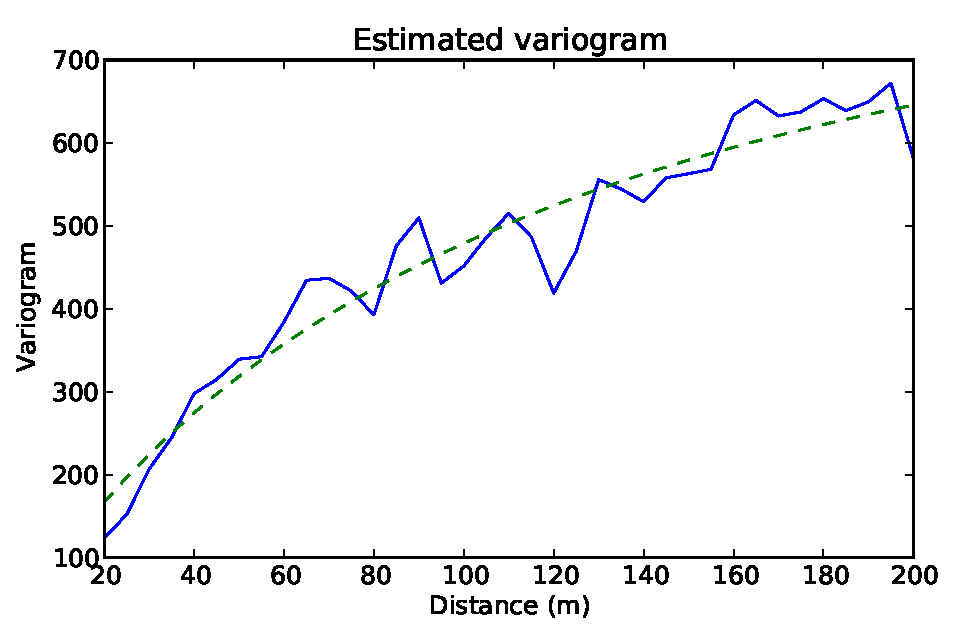
\includegraphics[width=\textwidth]{figures/stadium-variogram.pdf}
  \caption{An empirically estimated variogram model for \(h\) ranging from 20 to
    200 meters, in 5-meter increments, along with the fit model (dashed
    line). After 200 meters, the number of data points available to estimate the
    variogram becomes too small for reliable estimation.}
  \label{stadium-variogram}
\end{figure}

Since the kriging equations are expressed in terms of the covariance, we must
make use of Eq.~\ref{var-covar} to turn the estimated variogram into an
estimated covariance. This requires estimating \(\sigma_Y^2\), the variance of
the underlying random field. (The equations may be re-expressed in terms of the
variogram, but this also requires \(\sigma_Y^2\).)

To do so, we restate Eq.~\ref{var-covar} in terms of \(h\), the distance between
\(\mathbf{s}\) and \(\mathbf{s'}\), and take the limit:
\begin{equation}
  \lim_{h\to\infty} C(h) = \lim_{h\to\infty} \sigma_Y^2 - \gamma_Y (h)
\end{equation}
Of course, the covariance function goes to zero at infinite distance, under the
assumption of ergodicity. So we find that
\begin{equation}
\sigma_Y^2 = \lim_{h\to\infty} \gamma_Y(h),
\end{equation}
which is \(c\) in our chosen variogram model (Eq.~\ref{var-model}).

\section{Producing count rate maps}

A first step to implementing kriging for anomaly detection is to produce simple
maps of measured count rates. Python code implementing the above kriging system
was implemented using the SciPy library, which uses the LAPACK fast linear
algebra library to perform its operations. 

No matter how powerful the linear algebra library, it is still computationally
infeasible to solve Eq.~\ref{krige-system} on a consumer laptop when there are
several thousand data points to krige. We can give up some resolution and
instead aggregate our data into small spatial bins. In each spatial bin,
observations are summed and the total observation time computed; the resulting
aggregate data is then assigned the location of the ``center of mass''
(centroid) of the observations.

On datasets such as our Pickle Research Campus example data, a 20-meter bin
spacing produces reasonable results without requiring more than a minute or two
of calculation.

The kriging system is then used to create predicted count rates and variances
for each spatial grid point, and a contour plot made of the result. An example
is plotted in Fig.~\ref{prc-cps-contour} and Fig.~\ref{prc-cps-var-contour}.

\begin{figure}
  \centering
  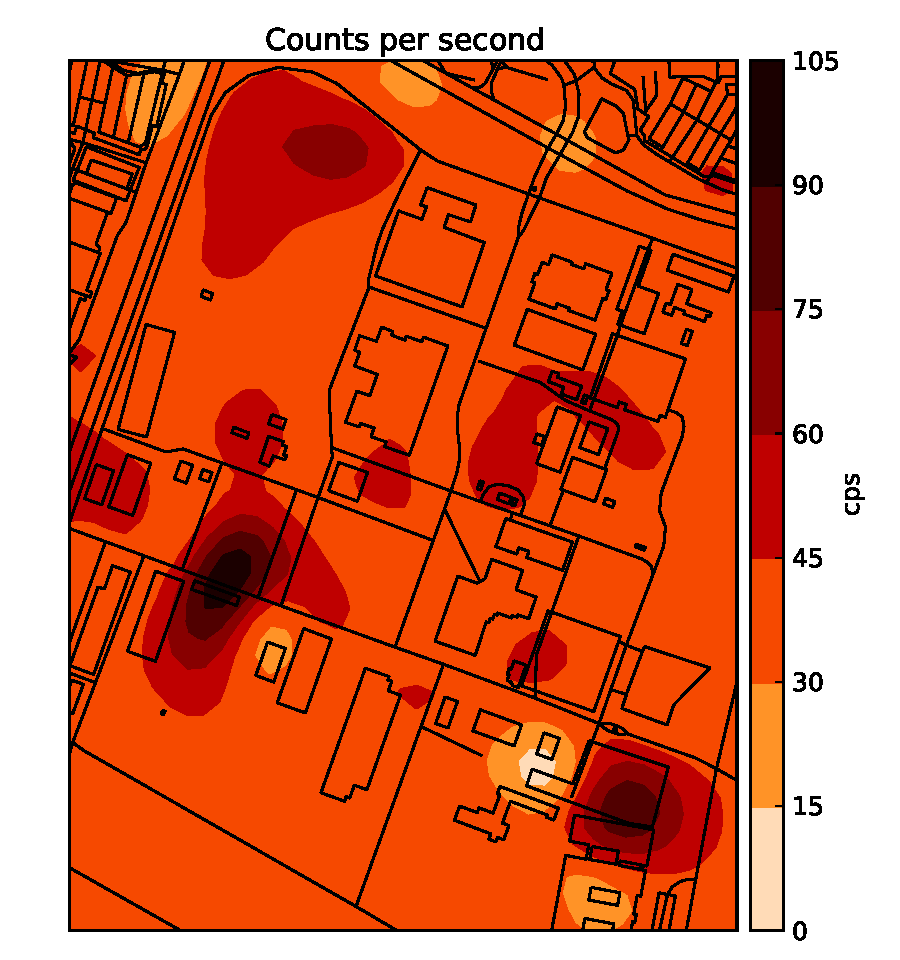
\includegraphics[width=0.8\textwidth]{figures/prc-cps-contour.pdf}
  \caption{Kriged mean count rates across the Pickle Research Campus during July
    2012. Compare against Fig.~\ref{prc-cps}. The same radioactive sources are visible.}
  \label{prc-cps-contour}
\end{figure}

\begin{figure}
  \centering
  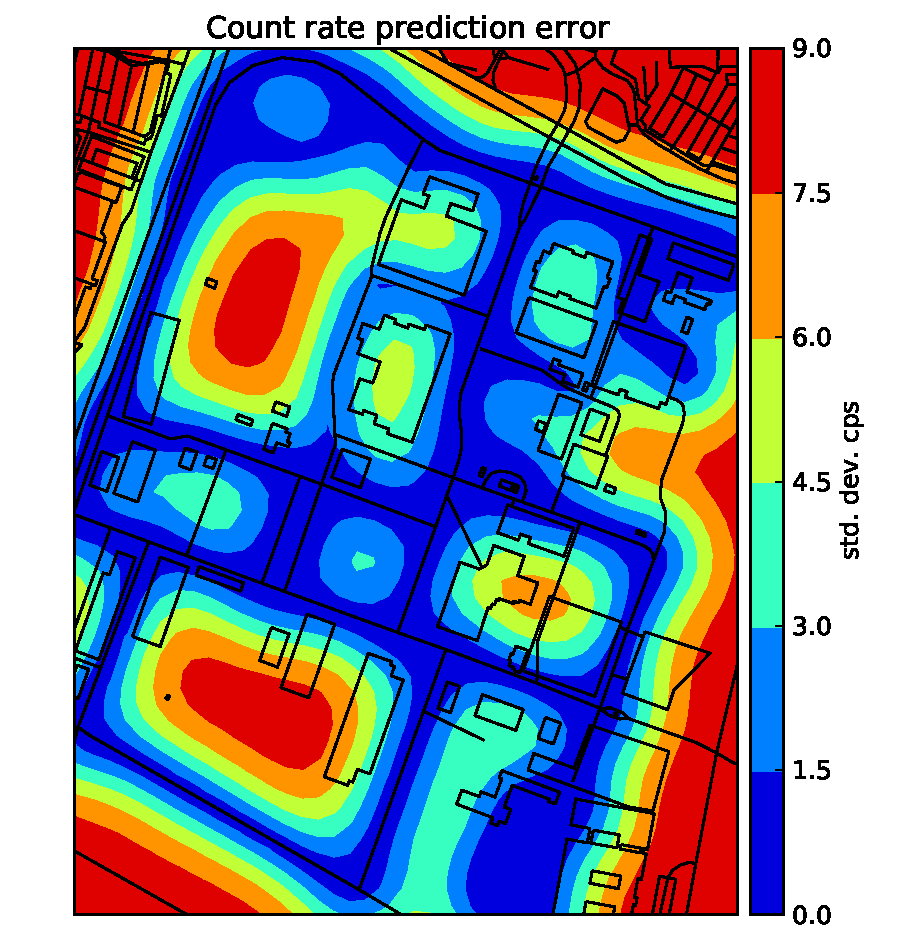
\includegraphics[width=0.8\textwidth]{figures/prc-cps-var-contour.pdf}
  \caption{Kriged prediction errors across the Pickle Research Campus in
    July 2012.}
  \label{prc-cps-var-contour}
\end{figure}

\section{Kriging anomaly detection}

\subsection{Anomaly mapping procedure}\label{krige-anomaly-mapping}

Anomaly detection emerges from kriging naturally. With Poisson kriging, we have
a system for mapping gamma count rates and producing predictions, with attached
variances, at any location. We may compare these predictions with new data to
see whether the new data is consistent with the past. In outline form, our
strategy is as follows:

\begin{enumerate}
  \item Collect a series of background observations in a region.
  \item Divide the region into spatial bins, as before, and perform kriging on
    the background observations to produce a prediction and matching prediction
    variance.
  \item Aggregate the new observations into spatial bins and compare the
    spectrum in each bin to the kriged prediction for that bin, producing a
    \(p\) value for the spectral difference.
  \item Produce a map of the \(p\) values.
\end{enumerate}

The first two steps are straightforward. But to perform steps 3 and 4, we need
an anomaly statistic.

\subsection{Count rate anomaly statistics}

Kriging provides us predictions and their prediction variance, which we must use
to determine if the new observations are consistent with the past. If we want
the predictive distribution of \(Z(\mathbf{s})\), the counts observed at some
new observation point, using the kriged prediction \(\hat Y(\mathbf{s})\), we
have:
\begin{align}
  Z(\mathbf{s}) | \hat Y(\mathbf{s}) t(\mathbf{s}) &\sim \text{Poisson}(\hat Y(\mathbf{s})
  t(\mathbf{s}))\\
  \hat Y(\mathbf{s}) t(\mathbf{s}) &\sim \text{Gamma}(a, (1-b)/b),
\end{align}
where \(t(\mathbf{s})\) is the observation time at the new point, and \(a\) and
\(b\) are chosen to match the mean and variance of the gamma distribution with
the prediction and prediction variance. In this case,
\(E[Y(\mathbf{s})t(\mathbf{s})] = t(\mathbf{s}) E[Y(\mathbf{s})]\) and
\(\text{var}(Y(\mathbf{s})t(\mathbf{s})) = t(\mathbf{s})^2
\sigma_Y^2\), so:
\begin{align}
  a &= \frac{\hat Y^2}{\sigma_{\hat Y}^2}\\
  b &= \frac{t(\mathbf{s}) \sigma_{\hat Y}^2}{\hat Y + t(\mathbf{s}) \sigma_{\hat Y}^2}.
\end{align}

Here \(\sigma_{\hat Y}^2\) is the prediction variance estimated by the kriging
procedure and \(\hat Y\) the predicted mean. With this information we can
compute the posterior predictive distribution of \(Z(\mathbf{s})\), our new
observation. For ease of integration, I substitute
\(x=Y(\mathbf{s})t(\mathbf{s})\):
\begin{equation}
P(Z(\mathbf{s})) = \int_0^\infty P(Z(\mathbf{s})|x) P(x) \, dx
\end{equation}
This integral is analytically tractable, and turns out to be a
negative binomial distribution with parameters \(a\) and \(b\):
\begin{equation}\label{post-predictive}
  Z(\mathbf{s}) \sim \text{NB}(a,b)
\end{equation}
We can use this to easily compute \(p\) values for our observed \(Z\), comparing
it to the predictions we derive from our background data.

\subsection{Detecting spectral anomalies}\label{spectral-anomaly}

The SCRAM algorithm aims to detect differences in spectral shape rather than
overall count rate, and we would like to replicate that behavior. To do this, we
divide the spectrum into bins as before, and krige the count rate in each bin
independently. (Cokriging may be more appropriate, because count rates in
separate energy bins are likely to be correlated; however, we did not explore
cokriging here.)  We then perform the count rate detection algorithm on each
energy bin in the spectrum.

Suppose there are \(n\) energy bins. We would like to know if any single bin has
an abnormally high count rate; to do this, we take the minimum \(p\) value out
of the \(n\) computed. Because \(p\) values are uniformly distributed on the
\((0,1)\) interval, the minimum of \(n\) is distributed as
\(\text{Beta}(1,n)\).\cite{David} Consequently we can compute an anomaly
statistic across all \(n\) bins by using the density of the beta distribution.

\subsection{Choosing an alarm threshold}

We will need to use a procedure to control false alarms. Typical hypothesis
testing provides bounds on the familywise error rate, which answers the question
``If there are no anomalies, how frequently will I falsely detect an anomaly?''
The simplest method is the Bonferroni correction, in which we set our
statistical significance criterion to be \(p < \alpha/n\), where \(n\) is the
number of tests performed. This method limits our statistical power, requiring a
high threshold of significance, though other more sophisticated techniques exist
with greater power.\cite{Holm:1979ws}

In a practical sense, though, we are not interested in the familywise error
rate. Operators of a radiation anomaly detection system are more concerned with
the false discovery rate: what proportion of alarms are false alarms?

The difference between familywise error rate and false discovery rate can be
seen by example. Suppose we test for anomalies each day, but true anomalies only
appear once every 1,000 days. If we control for a 1\% familywise error rate and
detect every single true anomaly, there will be 10 false positives and one true
positive.

In practical use, this is highly inconvenient. A system with too many false
positives is a system that will be ignored; each false positive incurs a cost to
investigate and dismiss. We would prefer the false discovery rate to be much
lower.

(Of course, there will be other sources of false positives beyond statistical
error: medical radioisotopes in recently treated patients, the transport of
industrial sources, and so on. Many of these can be mitigated with other
techniques, such as spectral analysis to determine the type of radioactive
source detected.)

We use the Benjamini-Hochberg procedure to control false discovery
rate.\cite{Benjamini:1995ws} We compute \(p\) values at many spatial points
following the procedure in Section~\ref{krige-anomaly-mapping}. Let the \(N\)
\(p\) values be denoted by \(P_{(1)}, P_{(2)}, \ldots, P_{(n)}\), sorted in
ascending order. Then, let \(k\) be the largest \(i\) such that
\begin{equation}
P_{(i)} \leq \frac{i}{N} q
\end{equation}
where \(q\) is the false discovery rate desired. We may reject all the
hypotheses where \(1 \leq i \leq k\). This is guaranteed to maintain a false
discovery rate of \(q\) or less.

This procedure will have higher statistical power than a procedure designed to
meet a certain false discovery rate goal while producing more useful results. In
one example case, we searched for anomalies in a map containing 138 kriged
points, most of which were true anomalies. Had we chosen to target an overall
false-positive rate of \(\alpha = 0.05\) using the Bonferroni correction, we
would have required \(p < 3.6\times 10^{-4}\); targeting \(q=0.05\), a much more
useful goal, allows searching for \(p < 0.12\), a factor of 319 difference. The
anomalies were successfully detected.

In another test, we searched for anomalies in a map containing 116 kriged points
in which there were no known true anomalies. The \(p\) criterion from the
Benjamini-Hochberg procedure was 5 times higher than that from the Bonferroni
correction, and even then, the system correctly reported no anomalies. One can
see how the Benjamini-Hochberg procedure adapts, choosing different criteria
based on the distribution of \(p\) values in the data.

Variations on the Benjamini-Hochberg procedure have been developed for the case
where the test statistics are dependent, which is the case
here.\cite{Benjamini:2001ho} The original procedure still works quite well in
this case, however, so we did not explore alternatives which account for the
dependency. Future work may seek to characterize the spatial dependence in
anomaly statistics and apply a suitable false discovery rate procedure.

It is also important to note that the Benjamini-Hochberg procedure has a
dependence on \(N\), the total number of hypotheses tested. If we choose to
krige over a region of a different size, or if we aggregate our data into
smaller spatial bins, \(N\) will vary and the significance level required for
detection will change. We must fix these parameters in advance for the procedure
to deliver its false discovery rate guarantees.

\section{Results}

\subsection{Simulation study}

Fig.~\ref{minimum-detectable} presents the minimum detectable source size at
various distances when using the SCRAM algorithm. We applied a similar procedure
to test the effectiveness of Poisson kriging anomaly detection.

The methods are not directly comparable due to their differing designs. The
SCRAM simulations aggregated the simulated data with an injected source and
computed a single anomaly statistic; Poisson kriging will aggregate the data
into much smaller spatial bins, using the covariance structure between spatial
bins for more accurate estimation, and will produce multiple test statistics.

We chose a procedure which is intended to mirror typical real-world use of
Poisson kriging anomaly detection:

\begin{enumerate}
  \item Inject a simulated cesium-137 source a fixed distance away from the
    roadway in a single day's observations at Pickle Research Campus.
  \item Perform kriging anomaly detection with 20-meter spatial bins across all
    of Pickle Research Campus, using a false detection rate of \(q = 0.05\).
  \item If one or more anomalies are reported along the stretch of road where
    the source has been injected, count this as a detection.
  \item If no anomalies are reported, increase the source size and repeat the
    simulation.
\end{enumerate}

The same dataset and sample spectra were used for source injection as in
Fig.~\ref{minimum-detectable}. Some results are given in
Table~\ref{krige-detectable}. These were computed with eight energy bins, as
described in Section~\ref{spectral-anomaly}. Two days of background data were
used, comprised of four data collection runs -- fewer than are generally
required for the SCRAM method. In general, the kriging procedure appears more
powerful than SCRAM: smaller radioactive sources are required to cause alarms,
and so a sensor system using Poisson kriging can detect sources of a given size
farther away than a SCRAM-based network.

\begin{table}
  \centering
  \begin{tabular}{r| c c}
    Distance (m) & SCRAM source (mCi) & Kriging source (mCi)
    \\\hline
    54 & 81 & 50\\
    98 & 256 & 175\\
    152 & 807 & 600
  \end{tabular}
  \caption{Minimum detectable source sizes at various distances from the road,
    for both the SCRAM and kriging anomaly detection systems. Kriging sizes are
    rough estimates.}
  \label{krige-detectable}
\end{table}

However, some false positives were detected by Poisson kriging, far away from
the region containing the injected source. Future work will be required to
determine the cause of these anomalies.

The Poisson kriging procedure's power increases when we consider overall count
rate rather than the count rate in eight separate energy bins, as we do not need
to perform the correction for using the minimum of eight \(p\) values. We are
interested in spectra rather than rates, however, and so this tradeoff may be
desired.

\subsection{Stadium data}

We also tested Poisson kriging on the football stadium data described in
Section~\ref{football}, using the three datasets collected with an empty stadium
as background data. Here the results were less satisfactory. When testing with a
\(q = 0.05\) false discovery rate and eight spectral bins, no anomalies were
detected in the October 20th data collection run, despite two being detected and
verified by SCRAM. Relaxing the significance requirements to \(q = 0.5\) did not
help. Switching to kriging total count rate improved detection performance so
that one of the known anomalies was detected at \(q=0.05\), while setting
\(q=0.25\) allowed both sources to be detected along with several false
positives.

These results contradict the simulation study, which showed that kriging anomaly
detection has superior detection performance. We hypothesize that this is due to
high prediction variance in the stadium dataset: using all available background
data, prediction standard deviations within the stadium vary between 4 and 12
counts per second, as compared to standard deviations of less than 1 in the
Pickle Research Campus data. The prediction variance determines the shape of the
posterior predictive distribution of \(Z(\mathbf{s})\)
(Eq.~\ref{post-predictive}), with a higher prediction variance resulting in a
wider predictive distribution.

The difference in prediction variance is partly a result of the greater amount
of data collected at Pickle Research Campus, but it also a result of the nature
of the background radiation at each location. The estimated variogram within the
stadium has a high variance \(\sigma_Y^2\), so prediction variances will
necessarily be higher (see Eq.~\ref{prediction-variance}). This is likely a
result of the systematic differences in count rate seen in different sections of
the stadium; see Section~\ref{football} and Fig.~\ref{stadium-heatmap}. In
addition, count rates were not always consistent between data collection runs
even when spectral shape remained constant. This may be due to detector
orientation and position as it was carried through the stadium.

Consequently we see the need for a kriging anomaly detection algorithm which is
completely independent of count rate, depending only on spectral shape. We also
see that the kriging model can be less effective in some areas where the kriging
system assumptions are violated. Operators of a kriging anomaly detection system
would have to be careful of this, locating areas with unusually high prediction
variance and adapting their search patterns to the lower system sensitivity.

\section{Future kriging steps}

Poisson kriging has not been fully developed for this application. Before the
system becomes practical, we must explore its performance in a number of
simulated and real tests, similar to the tests performed on the SCRAM system. We
must determine whether kriging provides significant benefits over SCRAM in a
wide range of operating environments.

We have not explored many potentially useful kriging techniques. We treat each
spectral bin independently when kriging, which ignores much of the structure in
spectral data -- count rates in separate bins tend to be correlated, as
radioactive sources may emit in several bins. Cokriging techniques should be
adapted to Poisson kriging and applied to spectral data to produce a more
powerful technique.

There are also cokriging techniques specifically designed to handle functional
data, such as gamma spectra.\cite{Nerini:2010ba,Giraldo:2010jx} These techniques
involve either treating observations of the spectrum as a large cokriging
problem or decomposing the spectrum into a small number of basis functions and
cokriging their coefficients. These techniques represent the structure inherent
in the data more closely, and may prove useful in spectral mapping.
